\documentclass[11pt]{article}


\usepackage[top=2cm, bottom=2cm, left=3.5cm, right=3.5cm]{geometry}
\usepackage{hyperref}       % hyperlinks
\usepackage{url}            % simple URL typesetting
\usepackage{booktabs}       % professional-quality tables
\usepackage{microtype}      % microtypography
\usepackage[table, dvipsnames, svgnames]{xcolor}  % colors
\usepackage[outline]{contour}% http://ctan.org/pkg/contour
\usepackage{wrapfig}
\usepackage{graphicx}
\usepackage{bm}
\usepackage{bbm}
\usepackage{multirow}
\usepackage{pifont}
\usepackage{rotating}
\usepackage{tikz}
\usepackage{amsmath}
\usepackage{amsfonts}
\newcommand{\xmark}{\ding{55}}%

\setlength{\tabcolsep}{3.5pt}

\hypersetup{
	colorlinks=true, %set true if you want colored links
	linktoc=all,     %set to all if you want both sections and subsections linked
	linkcolor=black,  %choose some color if you want links to stand out
	citecolor=cyan,
}




\allowdisplaybreaks



\newcommand{\defeq}{\vcentcolon=}
\newcommand{\im}{\operatorname{im}}
\newcommand{\Hom}{{\rm{Hom}}}
\newcommand{\diam}{{\rm{diam}}}
\newcommand{\dom}{\text{dom}}
\newcommand{\ovl}{\overline}
\newcommand{\rr}{\mathbb{R}}
\newcommand{\EE}{\mathcal{E}}
\newcommand{\VV}{\mathcal{V}}
\newcommand{\mystar}{{\fontfamily{lmr}\selectfont$\star$}}
\newcommand{\llangle}{\langle \langle}
\newcommand{\rrangle}{\rangle \rangle}

%bold commands
\newcommand{\xx}{\bm{x}}
\newcommand{\Xx}{\bm{X}}
\newcommand{\Tt}{\bm{T}}
\newcommand{\yy}{\bm{y}}
\newcommand{\ee}{\bm{e}}
\newcommand{\cc}{\bm{c}}
\newcommand{\uu}{\bm{u}}
\newcommand{\vv}{\bm{v}}
\newcommand{\ww}{\bm{w}}
\newcommand{\om}{\bm{\omega}}
\newcommand{\al}{\bm{\alpha}}
\newcommand{\be}{\bm{\beta}}
\newcommand{\si}{\bm{\sigma}}
\newcommand{\ta}{\bm{\tau}}


%calcommand

\newcommand{\mc}{\mathcal}

\DeclareMathOperator*{\argmax}{arg\,max}
\DeclareMathOperator*{\argmin}{arg\,min}

\setlength{\parindent}{0pt}

\author{Simone Manti, AU ID 734894, \texttt{smanti@mpe.au.dk} \\
	Final project for Neural Networks and Deep Learning 2024}

\title{Symbolic Model-Based Reinforcement Learning}



\begin{document}
	\maketitle

\section{Introduction}

\section{Model-Based Reinforcement Learning}
Reinforcement Learning (RL), contrarily to standard Supervised Learning, requires a continue interaction with data to update the policy. Usually, model-free RL is employed to optimize the policy, where the agent can only use the data sampled interacting with the real environment. In particular, RL algorithms with high sample complexity are non-manageable in a real-world scenario due to its cost. An alternative is presented by the so-called Model-Based Reinforcement Learning (MBRL) \textcolor{red}{cit}, where apart from optimizing policy the environment model must be learned. In real-world scenario, having an environment model drastically reduces the complexity of generating new training samples for RL algorithms.
In the following, we briefly overview the main components of MBRL. A more extensive treatment can be found in \textcolor{red}{put all the paper of MBRL}. 

MBRL restates the problem as a Markov Decision Process (MDP) \cite{puterman2014}. A MDP is a tuple $\{\mathcal{S}, \mathcal{A}, \mathcal{T}, \mathcal{R}, p(s_0), \gamma\}$, \textcolor{red}{continue from Model-Based Reinforcement Learning: A Survey}.

\section{Symbolic Regression}

\section{Experiments and implementations details}

\subsection{Simple 1-dimensional MDP}


\begin{figure}
	\centering
	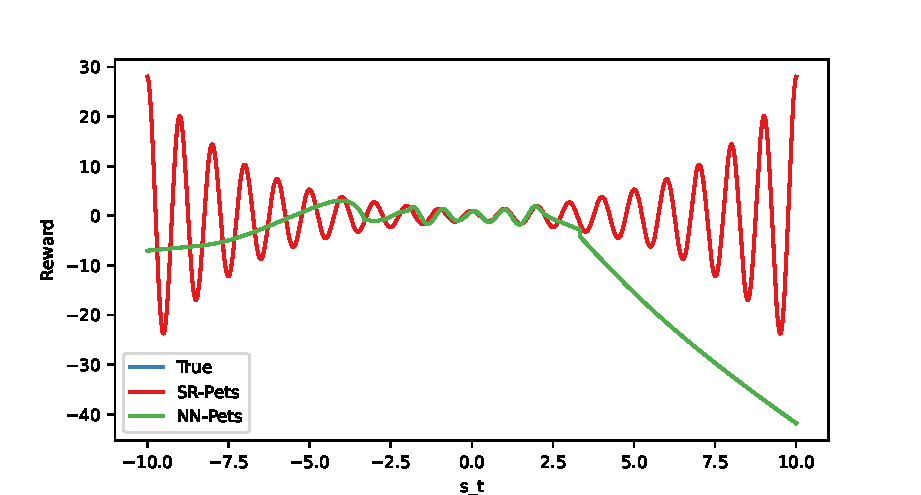
\includegraphics{simple1dmdp_pets.pdf}
	\caption{??}
\end{figure}

\subsection{Cartpole}


\section{Conclusion and discussion}

\section*{References}

\bibliographystyle{ieeetr}
\begin{thebibliography}{10}
	\bibitem{puterman2014}
	M. L.~Puterman, ``Markov Decision Processes: Discrete Stochastic Dynamic Pro-
	gramming.'' {\em John Wiley and sons}, 2014.
	
\end{thebibliography}
\end{document}